% !TeX spellcheck = es_ES
\documentclass[12pt, titlepage]{article}
\usepackage[nottoc,notlot,notlof,numbib]{tocbibind}
\usepackage[letterpaper, margin=2.5cm]{geometry}
\usepackage[utf8]{inputenc}
\usepackage[spanish]{babel}
\usepackage{listings}
% imagenes
\usepackage{graphicx} 
\usepackage{float}
% fin imagenes
\usepackage{url}
\usepackage{color}
\usepackage{amsmath}
\usepackage{bm}

\definecolor{dkgreen}{rgb}{0,0.6,0}
\definecolor{gray}{rgb}{0.5,0.5,0.5}
\definecolor{mauve}{RGB}{253,151,31}
\definecolor{deepred}{RGB}{249,38,114}

\lstset{frame=tb,
	language=MATLAB,
	aboveskip=3mm,
	belowskip=3mm,
	showstringspaces=false,
	columns=flexible,
	numbers=left,
	stepnumber=1,
	basicstyle={\small\ttfamily},
	numberstyle=\tiny\color{gray},
	keywordstyle=\color{blue},
	commentstyle=\color{dkgreen},
	stringstyle=\color{mauve},
	breaklines=true,
	breakatwhitespace=true,
	tabsize=2,
	morekeywords={self, append},
	emph={},
	emphstyle=\color{deepred}
}

\title{Reporte Perceptron simple}
\author{Barrera Pérez Carlos Tonatihu \\Boleta: 2016630023\\ Profesor: Moreno Armendariz Marco Antonio \\ Redes Neuronales \\ Grupo: 3CM2 }
\begin{document}
    \maketitle
    \tableofcontents
    \newpage
    \section{Introducción}
    El siguiente trabajo contiene conceptos fundamentales en el estudio del perceptron como lo son su modelo matemático y arquitectura al igual que el algoritmo de aprendizaje que realiza. Además, para poder apreciar estos conocimientos teóricos se programo un perceptron simple que puede clasificar hasta 4 diferentes clases.
    \\\\
    En este se introdujeron diferentes conjuntos de entrenamiento para poder ver como trabaja el perceptron para diferentes tamaños de problema. De igual forma se realizo un análisis de los datos obtenidos y de las gráficas correspondientes a cada experimento para tratar de entender que es lo que sucedió y el porqué paso.
    \\\\
    Al final se incluye una conclusión a todo el reporte, principalmente a los resultados experimentales para poder obtener puntos claves que fueron resultado de estas pruebas y entender de una mejor forma las ventajas y desventajas que tiene el perceptron así como sus limitaciones. De igual forma se anexa la bibliografía consultada y el código que se desarrollo para la práctica.
    \newpage
    \section{Marco teórico}
    El perceptron fue desarrollado en los años cincuenta por un grupo de investigadores entre los que estaba Frank Rosenblantt, la principal característica de esta red es que utiliza un algoritmo de aprendizaje supervisado esto quiere decir que se le tiene que dar ejemplos de como operar (conjunto de entrenamiento), este conjunto de entrenamiento tiene la siguiente forma:
    \[ \left\lbrace \boldsymbol{p_1, t_1}\right\rbrace , \left\lbrace \boldsymbol{p_2, t_2}\right\rbrace , ... , \left\lbrace \boldsymbol{p_Q, t_Q}\right\rbrace  \]
    en donde cada par esta formado por un vector de entrada $\boldsymbol{p_q}$ y un vector objetivo $\boldsymbol{t_q}$ que es la salida correspondiente a dicho vector de entrada. \cite{libro1}
    Además, la arquitectura del perceptron es la siguiente:
    \begin{figure}[H]
        \begin{center}
            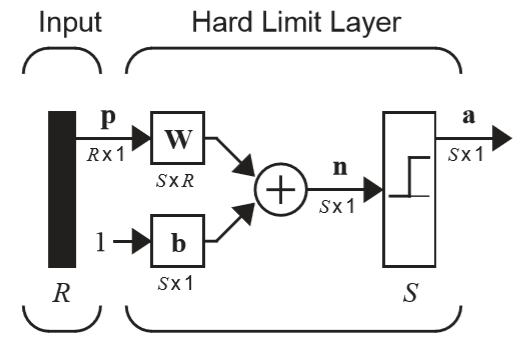
\includegraphics[width=7cm]{img/perceptron/perceptron.png}
            \caption{Arquitectura de un perceptron simple. \cite{libro1}}
            \label{fig:perpectron-diagrama}
        \end{center}
    \end{figure}
    Debido a que utiliza una función \emph{hardlim} la salida de la red solo puede tener dos posibles valores el cual esta definido por $\boldsymbol{a = hardlim(Wp+b)}$. El hecho de que solo tenga dos valores es lo que nos permite establecer una frontera de decisión entre dos clases como la de la figura \ref{fig:frontera}, esto en consecuencia de que cada neurona puede clasificar 2 diferentes clases.
    \begin{figure}[H]
        \begin{center}
            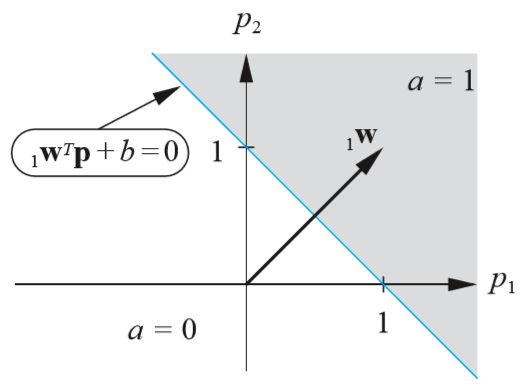
\includegraphics[width=8cm]{img/perceptron/frontera.png}
            \caption{Ejemplo de una frontera de decisión. \cite{libro1}}
            \label{fig:frontera}
        \end{center}
    \end{figure}
    Dicha frontera es determinada por un valor de entrada para el cual la salida de la red es 0, es decir,
    \[\boldsymbol{Wp+b} = 0 \]
    Como se menciono antes, el perceptron utiliza una regla de aprendizaje que se basa en la modificación de los pesos y bias con base a un error a lo largo de la propagación hacia adelante que se realiza. 
    Para lograr esto se sigue el siguiente algoritmo.\cite{otro}
    \begin{enumerate}
        \item Se tiene el conjunto de entrenamiento
        \[ \left\lbrace \boldsymbol{p_1, t_1}\right\rbrace , \left\lbrace \boldsymbol{p_2, t_2}\right\rbrace , ... , \left\lbrace \boldsymbol{p_Q, t_Q}\right\rbrace\]
        \item Se inicializan los valores de $\boldsymbol{W}$ y $\boldsymbol{b}$ con valores aleatorios pequeños.
        \item Procedemos a hacer la propagación hacia adelante de un vector prototipo, es decir, evaluamos un $\boldsymbol{p_Q}$ en nuestra red de la forma.
        \[ \boldsymbol{a = hardlim(Wp_Q+b)} \]
        \item Lo siguiente es obtener el error comparando el valor objetivo asociado a dicho vector prototipo con la salida producida por la red
        \[ \boldsymbol{e=t-a} \]
        \item A continuación aplicamos el aprendizaje correspondiente al bias y matriz de pesos de nuestra red. Es decir, el nuevo valor de nuestra matriz de pesos sera igual al valor actual más el producto del error obtenido en el paso por la transpuesta del vector de entrada que se utilizo.
        \[ \boldsymbol{W^{nueva} = W^{vieja} + ep^{t}} \]
        Para el caso del bias tenemos algo similar solo que el nuevo valor de $\boldsymbol{b}$ sera igual al valor actual más el error producido.
        \[ \boldsymbol{b^{nueva} = b^{vieja} + e} \]
        \item Esto se realiza para cada elemento del conjunto de entrenamiento para poder completar una iteración.
        \item Este procedimiento se realiza hasta que cada salida de la red con cada vector de entrada sea igual a su correspondiente objetivo $a_Q = t_Q$ o en el caso de que se alcance un máximo de iteraciones.
    \end{enumerate}
\newpage
\section{Resultados experimentales}
Para hacer las pruebas correspondientes sobre el perceptron se introdujo un archivo de texto en donde se encontraba el conjunto de entrenamiento que se utilizaría, además a la red se le indicaba cual es el numero máximo de iteraciones si es que no lograba hacer que la salida fuera igual al respectivo vector objetivo encontrado en el conjunto de entrenamiento.

\begin{figure}[H]
    \begin{center}
        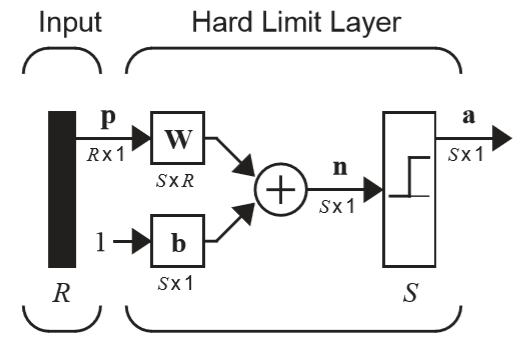
\includegraphics[width=8cm]{img/perceptron/perceptron.png}
        \caption{Arquitectura de un perceptron simple. \cite{libro1}}
        \label{fig:perpectron-diagrama2}
    \end{center}
\end{figure}

Los valores de los pesos y bias finales son almacenados en un archivo llamado resultado\_hora\_fecha.txt además de que se grafican la evolución de estos valores junto a el error que se tuvo a lo largo de todas las iteraciones.
\\
\textbf{Experimento 1}
El conjunto de entrenamiento que se utilizo en este caso fue.
\[ \left\lbrace \boldsymbol{p_1} = \left[\begin{array}{c} 0\\ 0\end{array}\right], t_1 = 0  \right\rbrace, \left\lbrace \boldsymbol{p_2} = \left[\begin{array}{c} 0\\ 1\end{array}\right], t_2 = 0  \right\rbrace, \left\lbrace \boldsymbol{p_3} = \left[\begin{array}{c} 1\\ 0\end{array}\right], t_3 = 0  \right\rbrace, \left\lbrace \boldsymbol{p_4} = \left[\begin{array}{c} 1\\ 1\end{array}\right], t_4 = 1  \right\rbrace  \]
Este conjunto de entrenamiento de dos clases que produciría que el numero de neuronas del perceptron fuera 1 corresponde a la compuerta AND de dos entradas. Por lo que los valores asociados a nuestra arquitectura de la figura \ref{fig:perpectron-diagrama2} fueran los siguientes.
\begin{align*}
S=1 && R=2
\end{align*}
Además los valores asociados a $\boldsymbol{W}$ y $\boldsymbol{b}$ fueron números aleatorios pequeños. Mientras que el numero de iteraciones máximas fue $it_{max}=50$.
\begin{figure}[H]
    \begin{center}
        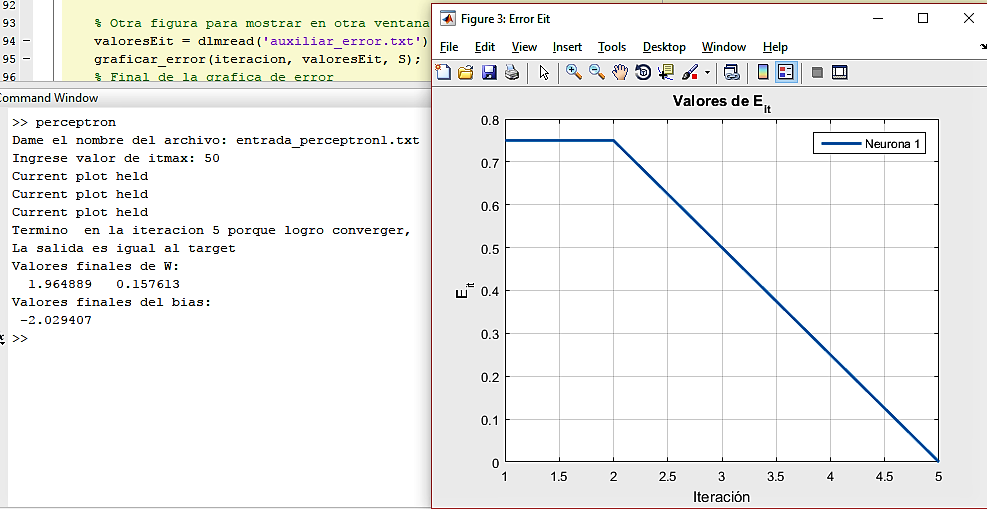
\includegraphics[width=15cm]{img/perceptron1/error.png}
        \caption{Evolución del error a lo largo de las iteraciones de la prueba 1.}
        \label{fig:error1}
    \end{center}
\end{figure}
En la figura \ref{fig:error1} se puede observar que la red llego a un resultado en la iteración 5 debido a que logro converger lo que quiere decir que las salidas fueron igual a sus respectivos vectores objetivo. De esta forma los valores de pesos y bias finales fueron los siguientes.

\begin{align*}
\boldsymbol{W} = \left[\begin{array}{cc}1.964889 & 0.157613\end{array}\right] && \boldsymbol{b} = -2.029407
\end{align*}

La evolución de estos valores se puede observar en la figura \ref{fig:pesosbias} además de que los valores finales son almacenados en su respectivo archivo \emph{resultado\_hora\_fecha.txt}.
\begin{figure}[H]
    \begin{center}
        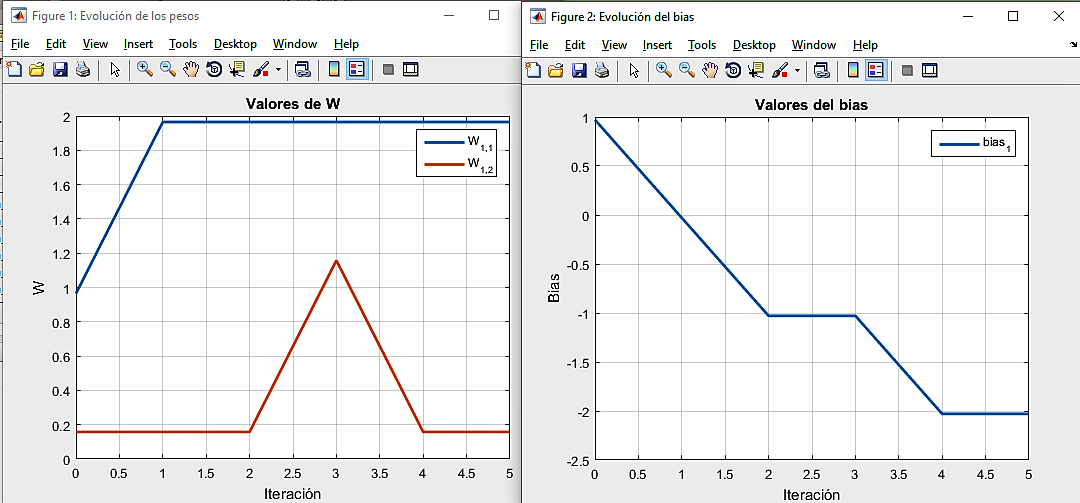
\includegraphics[width=15cm]{img/perceptron1/pesosbias.png}
        \caption{Evolución de pesos y bias de la prueba 1.}
        \label{fig:pesosbias}
    \end{center}
\end{figure}
\textbf{Experimento 2}
El conjunto de entrenamiento que se utilizo para entrenar a la red fue.
\[ \left\lbrace \boldsymbol{p_1} = \left[\begin{array}{c} 1\\ 1\end{array}\right], \boldsymbol{t_1} = \left[\begin{array}{c} 0\\ 0\end{array}\right]  \right\rbrace, \left\lbrace \boldsymbol{p_2} = \left[\begin{array}{c} 2\\ 0\end{array}\right], \boldsymbol{t_2} = \left[\begin{array}{c} 0\\ 0\end{array}\right]  \right\rbrace, \left\lbrace \boldsymbol{p_3} = \left[\begin{array}{c} -1\\ -1\end{array}\right], \boldsymbol{t_3} = \left[\begin{array}{c} 0\\ 1\end{array}\right]  \right\rbrace,\]

\[ \left\lbrace \boldsymbol{p_4} = \left[\begin{array}{c} 0\\ -1\end{array}\right], \boldsymbol{t_4} = \left[\begin{array}{c} 0\\ 1\end{array}\right]  \right\rbrace, \left\lbrace \boldsymbol{p_5} = \left[\begin{array}{c} -2\\ 0\end{array}\right],\boldsymbol{t_5} = \left[\begin{array}{c} 1\\ 0\end{array}\right]  \right\rbrace, \left\lbrace \boldsymbol{p_6} = \left[\begin{array}{c} -1\\ 1\end{array}\right], \boldsymbol{t_6} = \left[\begin{array}{c} 1\\ 0\end{array}\right]  \right\rbrace,\]

\[ \left\lbrace \boldsymbol{p_7} = \left[\begin{array}{c} 0\\ 2\end{array}\right], \boldsymbol{t_7} = \left[\begin{array}{c} 1\\ 1\end{array}\right]  \right\rbrace, \left\lbrace \boldsymbol{p_8} = \left[\begin{array}{c} 1\\ 2\end{array}\right], \boldsymbol{t_8} = \left[\begin{array}{c} 1\\ 1\end{array}\right]  \right\rbrace\]
Es por estos valores que las dimensiones de la red mostrada en la figura \ref{fig:perpectron-diagrama2} quedan definidas de la siguiente forma.
\begin{align*}
S = 2 && R = 2
\end{align*}
Lo cual crea una matriz de pesos de $2x2$ y una matriz de bias de $2x1$ con valores aleatorios pequeños y el número máximo de iteraciones es establecido como $it_{max}=50$.
\begin{figure}[H]
    \begin{center}
        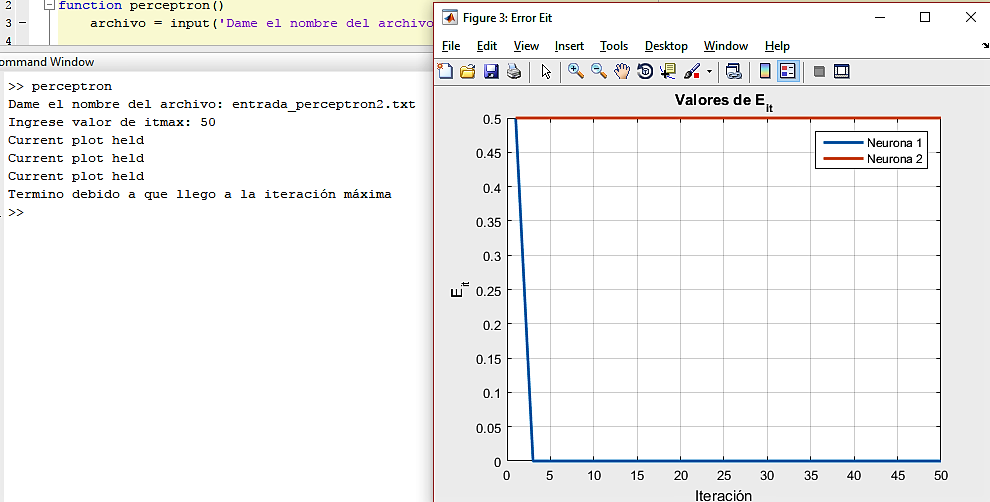
\includegraphics[width=15cm]{img/perceptron2/error.png}
        \caption{Evolución del error a lo largo de las iteraciones del experimento 2.}
        \label{fig:error2}
    \end{center}
\end{figure}
En este experimento la red no pudo dar un resultado satisfactorio y termino debido a que llego a la iteración máxima como se puede observar en la figura \ref{fig:error2}.

A pesar de esto, la gráfica de la evolución de pesos y bias que se encuentra en la figura \ref{fig:pesosbias2} es mostrada para poder ver el comportamiento tan peculiar que tuvo este caso.

\begin{figure}[H]
    \begin{center}
        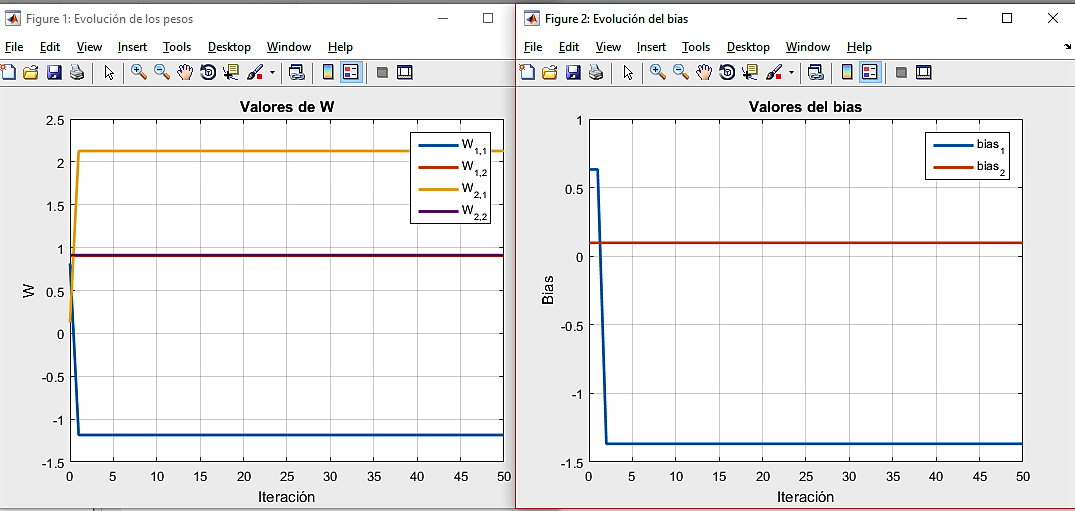
\includegraphics[width=15cm]{img/perceptron2/pesosbias.png}
        \caption{Evolución de pesos y bias del experimento 2.}
        \label{fig:pesosbias2}
    \end{center}
\end{figure}
\newpage
    \section{Discusión de resultados}
    En estos experimentos tuvimos un resultado satisfactorio y un experimento que no pudo converger, aun así, es interesante observar el comportamiento de las gráficas y el como en algunas iteraciones ocurren cambios de comportamiento demasiado drásticos, esto se puede ver tanto en las gráficas de error como en la de pesos y bias. Además de que la forma en la que se modifican los pesos no parece tener un comportamiento claro a diferencia del bias que en ambos experimentos fue disminuyendo en cada iteración hasta estabilizarse.
    
    Esto podría se consecuencia que las fronteras que se tratan de modelar se encuentran demasiado cercanas a los vectores que estamos utilizando lo que tiene como consecuencia que se genere ruido en el perceptron lo cual es la principal desventaja de utilizar este tipo de arquitectura.
    \newpage
     \section{Conclusiones}
     La principal ventaja que tenemos al usar el perceptron es que es una arquitectura bastante sencilla al igual la regla de aprendizaje que se utiliza para modificar los pesos y bias de la red. Es evidente que funciona muy bien para problemas en donde los vectores prototipo están lo suficientemente separados uno del otro como en el caso de la compuerta AND de dos entradas, pero en casos donde tengamos clases donde su separación no sea tan amplia tendremos el problema de trazar una correcta frontera de decision.
     
     Además que la frontera de decision es una desventaja que tiene el perceptron en si debido a que solo podremos trabajar con problemas linealmente separables como los tratados en este caso.
     \newpage
    \bibliographystyle{apalike}
    \bibliography{bibliografia}
    \newpage
    \section{Anexo}
    \begin{lstlisting}
%% Proceso de aprendizaje
function perceptron()
    archivo = input('Dame el nombre del archivo: ', 's');
    
    prueba = fopen(archivo, 'r');
    S = 0;
    targets = [];
    prototipos = [];
    R = 0;
    dimen = [];
    tipo_lectura = 0;
    while feof(prueba) == 0
        linea = fgetl(prueba);
        % Si no tiene llave es que es de dos clases y usamos una neurona
        if linea ~= '{'
            fclose(prueba);
            datos = dlmread(archivo);
            tam = size(datos);
            S = 1;
            prototipos = datos(:, 1:tam(2)-1)';
            dimen = size(prototipos);
            targets = datos(:, tam(2))';
            R = dimen(1);
            tipo_lectura = 1;
            break; % No tiene caso leer mas lineas
        else
            linea = linea(2:length(linea)-1);
            proto = linea(2:find(linea==',')-2);
            tar = linea(find(linea==',')+2:length(linea)-1);
            proto = str2num(proto);
            tar = str2num(tar);
            prototipos = [prototipos proto'];
            targets = [targets tar'];
        end
    end
    % Si tiene mas de dos clases
    if tipo_lectura == 0
        S = 2;
        dimen = size(prototipos);
        R = dimen(1);
    end   
    itmax = input('Ingrese valor de itmax: ', 's'); %5
    itmax = str2double(itmax);
    
    W = rand(S, R);
    b = rand(S, 1);
    
    auxiliar_w = fopen('auxiliar_w.txt', 'w');
    auxiliar_bias = fopen('auxiliar_bias.txt', 'w');
    auxiliar_error = fopen('auxiliar_error.txt', 'w');
    fprintf(auxiliar_w, '%.10f ', W);
    fprintf(auxiliar_w, '\n');
    
    fprintf(auxiliar_bias, '%.10f ', b);
    fprintf(auxiliar_bias, '\n');
    for iteracion = 1:itmax
        error = 0;
        for i = 1:dimen(2)
            p = prototipos(:, i);
            a = hardlim(W*p + b);
            e = targets(:, i) - a;
            W = W + (e*p');
            b = b + e;
            error = error + abs(e);
        end
        error = 1/dimen(2) * error;
    
        fprintf(auxiliar_w, '%.10f ', W);
        fprintf(auxiliar_w, '\n');
        
        fprintf(auxiliar_bias, '%.10f ', b);
        fprintf(auxiliar_bias, '\n');
        
        fprintf(auxiliar_error, '%.10f ', error);
        fprintf(auxiliar_error, '\n');
    
        if error == 0
            break;
        end
    end
    
    fclose(auxiliar_error);
    fclose(auxiliar_w);
    fclose(auxiliar_bias);
    
    % Figura de los valores de W
    valoresW = dlmread('auxiliar_w.txt');
    valores_bias = dlmread('auxiliar_bias.txt');
    graficar_pesos(valoresW, iteracion, S, R);
    graficar_bias(valores_bias, iteracion, S);
    % Final de la grafica de W
    
    % Otra figura para mostrar en otra ventana
    valoresEit = dlmread('auxiliar_error.txt');
    graficar_error(iteracion, valoresEit, S);
    % Final de la grafica de error
    
    % Criterio de terminacion
    if iteracion == itmax
        disp('Termino debido a que llego a la iteracion maxima');
    else
        fprintf('Termino  en la iteracion %d porque logro converger, ', iteracion);
        fprintf('\nLa salida es igual al target\n');
    
        % Desplegar valores finales de pesos y bias
        % Almacenar pesos y bias en archivo resultado_hora_fecha.txt
        fprintf('Valores finales de W: \n');
        fprintf('%10f ', W);
        fprintf('\n');
        
        fprintf('Valores finales del bias: \n');
        fprintf('%10f ', b);
        fprintf('\n');
    end
    % Final del criterio de terminacion
    
    archivo_final = strcat('resultado_', datestr(now, 'HH-MM_dd-mm-yyyy'));
    archivo_final = strcat(archivo_final, '.txt');
    finales = fopen(archivo_final, 'w');
    fprintf(finales, 'Valores finales de W: \n');
    fprintf(finales, '%.10f ', W);
    fprintf(finales, '\n');
    
    fprintf(finales, 'Valores finales del bias: \n');
    fprintf(finales, '%.10f ', b);
    fprintf(finales, '\n');
    fclose(finales);
end

%% graficar_bias
function graficar_bias(valores_bias, iteracion, S)
    figure('Name', 'Evolucion del bias');
    % Grafica un vector en x y otro vector en y
    plot(0:iteracion, valores_bias, 'LineWidth', 2); 
    hold;
    grid;
    % Etiquetas de los ejes
    xlabel('Iteracion');
    ylabel('Bias');
    % Titulo de nuestra grafica
    etiquetas = cell(1, S);
    for i = 1:S
        etiquetas{i} = ['bias_' num2str(i)];
    end
    legend(etiquetas);
    title('Valores del bias');
end
%% graficar_pesos: function description
function graficar_pesos(valoresW, iteracion, S, R)
    figure('Name', 'Evolucion de los pesos');
    % Grafica un vector en x y otro vector en y
    plot(0:iteracion, valoresW, 'LineWidth', 2); 
    hold;
    grid;
    % Etiquetas de los ejes
    xlabel('Iteracion');
    ylabel('W');
    
    etiquetas = cell(1, S*R);
    k = 1;
    for i = 1:S
        for j = 1:R
            etiquetas{k} = ['W_{' num2str(i) ',' num2str(j) '}'];
        k = k+1;
        end
    end
    legend(etiquetas);
    title('Valores de W');
end

%% graficar_error: function description
function graficar_error(iteracion, valoresEit, S)
    figure('Name', 'Error Eit');
    x = 1:iteracion;
    % Grafica un vector en x y otro vector en y
    plot(x, valoresEit, 'LineWidth', 2);
    hold;
    grid;
    % Etiquetas de los ejes
    xlabel('Iteracion');
    ylabel('E_{it}');
    % Titulo de nuestra grafica
    etiquetas = cell(1, S);
    for i = 1:S
        etiquetas{i} = ['Neurona ' num2str(i)];
    end
    legend(etiquetas);
    % Titulo de nuestra grafica
    title('Valores de E_{it}');
end
    \end{lstlisting}
\end{document}